\documentclass[a4paper,11pt]{article}
  % Métadonnées
  \title{Génération procédurale de contenu personnalisée selon le style de jeu et la personnalité du joueur}
  \author{Lecoq Simon (LECS09129600)}
  \date{}
  % Packages
  \usepackage{indentfirst}
  \usepackage{lmodern,amsmath}
  \usepackage[hyphens]{url}
  \usepackage{tabularx,array,arydshln}
  \usepackage{tikz}
  \usepackage[font=small,labelfont=bf]{caption}
  \usepackage[french]{babel}
  \usetikzlibrary{shapes.misc,arrows.meta,positioning,calc}
  % Corps du document
  \begin{document}
    % Titre
    \maketitle
    % Style
    \setlength{\parskip}{1em}

    % I - CONTEXTE
    \section{Contexte}\label{section:context}
  
      % Courte introduction sur les jeux vidéo
      L'industrie des jeux vidéo est un secteur d'activité qui représente une part importante dans l'univers du divertissement.
      Estimé à une valeur de 78 milliards de dollars en 2017, le marché des jeux vidéo devrait atteindre les 90 milliards d'ici 2020 avec 2.5 milliards de joueurs (en incluant les joueurs occasionnels)\footnote{2018 Video Game Industry Statistics, Trends \& Data : \url{wepc.com/news/video-game-statistics/}}.
      Démocratisés dans les années 1980 grâce à l'apparition des bornes d'arcades et l'arrivée des premières consoles de jeux \cite{Wolf}, et plus encore avec l'avènement des jeux mobiles au début des années 2010 grâce aux ordiphones, les jeux vidéo font désormais partie intégrante de la culture populaire.
    
      % Coûts de développement et ressources
      Avec les avancées technologiques, l'attente du public n'a cessé de croître et il n'est pas rare que le développement d'un jeu vidéo nécessite le travail de plusieurs dizaines, voire centaines de personnes, afin de mener à bien la conception, le développement, la direction artistique, le doublage, le marketing, etc.
      Inéluctablement, les coûts de production ont eux aussi augmenté, allant parfois même jusqu'à rivaliser avec l'industrie hollywoodienne : 
      la réalisation de \textit{Grand Theft Auto V} \cite{game:GTAV}, qui est le fruit de 5 années de travail mobilisant plus de 300 personnes, est estimé à un coût total de 250 millions de dollars (dont 137 millions uniquement pour le développement)\footnote{Un analyste indique que le développement de \textit{GTA V} a coûté plus de 137 millions de dollars : \url{gamesindustry.biz/articles/2013-02-01-gta-v-dev-costs-over-USD137-million-says-analyst}}.

      % Public cible élargi
      Pour compenser les coûts importants et rentabiliser leurs produits, la solution la plus évidente pour les producteurs de jeux vidéo est d'élargir le public cible.
      Afin d'étendre la démographie potentiellement intéressée, il convient de prendre en considération l'âge, le genre, la personnalité, la culture, etc. des joueurs.
      Par exemple, dans le jeu \textit{Splatoon 2} \cite{game:Splatoon2}, les terrains et modes de jeux suivent une rotation imposée par les développeurs ce qui convient aux joueurs japonais, mais qui ce peut frustrer les joueurs occidentaux, y voyant ici une contrainte\footnote{Un concepteur de Nintendo explique pourquoi le \textit{Salmon Run} n'est pas toujours disponible : \url{kotaku.com/nintendo-designer-explains-why-salmon-run-isnt-always-a-1801065018}}. 
      L'exemple présenté illustre le fait qu'il est difficile d'espérer pouvoir satisfaire entièrement un large public aussi varié sans adapter certains aspects du jeu pour correspondre aux attentes des joueurs.
          
      % Pose le problème sur lequel va porter la question de recherche
      La situation actuelle ne permet donc plus la création à la main de nouveau contenu original à la cadence espérée par les joueurs et pour tous les types de joueurs, en raison des goulots d'étranglement liés aux manques de ressources humaines, financières ou temporelles \cite{Hendrikx}.
      Il est donc nécessaire pour les concepteurs de jeux vidéo de trouver des méthodes permettant de réduire l'impact de ces limitations.
      
      % Introduction de la génération procédurale de contenu
      La Génération Procédurale de Contenu (GPC, définie dans la section \ref{section:defs-pcg}) est un moyen qui peut potentiellement être utilisée afin de combler le déficit de ressources du côté des créateurs de jeux.
      Si l'on se concentre sur les applications de la GPC en jeux vidéo, elle peut notamment être utilisée pour générer de nouvelles mécaniques de jeu, des quêtes, des armes, des dialogues, des environnements, des textures, etc. \cite{Togelius}, tout ceci dépendant ultimement de comment les concepteurs choisissent de l'implémenter et de s'en servir.
      
      % Exemple de No Man's Sky
      Par exemple, dans \textit{No Man's Sky} \cite{game:NoMansSky} (voir Figure \ref{fig:pcg}), la GPC fait partie intégrante des mécaniques de jeux et est utilisé afin de générer un univers immense contenant plusieurs trillions de planètes à explorer, chacune peuplée d'une faune et d'une flore générées également de façon procédurale. 
      Le contenu disponible aurait débouché sur des coûts prohibitifs s'il avait été entièrement réalisé à la main, cependant la GPC a permis de limiter de façon significative le nombre de ressources nécessaire à la création de celui-ci.

      % Figure GPC
      \begin{figure}
        \centering
        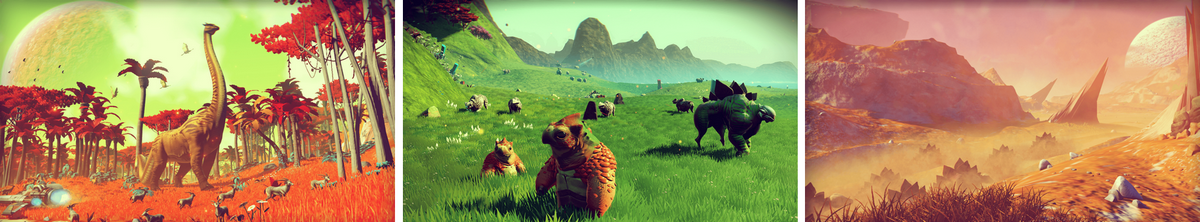
\includegraphics[width=\textwidth]{fig1.png}
        \caption{Exemples d'environnements générés par GPC. Images tirées du kit de presse du jeu \textit{No Man's Sky}\cite{game:NoMansSky}.}
        \label{fig:pcg}
      \end{figure}

      % Limitation de la GPC
      Reste que si le contenu générable est supposément infini grâce à la GPC, il n'est utile que s'il plaît aux joueurs, l'un des buts premiers des jeux vidéo étant le divertissement.
      Cette lourde responsabilité est attribuée aux concepteurs eux-mêmes, toutefois l'utilisation de la GPC requiert de faire << confiance >> à l'ordinateur en lui déléguant une partie du processus de création \cite{Riedl}.  
      
      % Introduction de la personnalisation dans les jeux
      Pour s'assurer que le contenu généré plaît au joueur, une des solutions envisageables est de s'inspirer du concept de << jeu personnalisé >> \cite{Bakkes}.
      En somme, cela consiste à réaliser un jeu qui exploite des modèles du joueur afin d'optimiser l'expérience de jeu du joueur en question.
      La personnalisation individuelle devrait (à condition d'être correctement exécutée) résulter sur des jeux avec des joueurs plus engagés, mieux divertis et globalement plus satisfaits \cite{Bakkes}.
      Dans la suite de ce papier, cette notion de << jeu personnalisé >> est explorée plus en profondeur.


    % II - PREREQUIS ET DEFINITIONS
    \section{Prérequis et définitions}\label{section:defs}

      Avant de discuter plus en détails la question de recherche, cette section définit plusieurs termes qui sont utilisés dans la suite de ce papier.
      
      % Contenu et expérience de jeu
      \subsection{Expérience de jeu}\label{section:defs-pem}

        Ce papier reprend la définition de Yannakakis et al. (2015) \cite{Yannakakis} pour expliquer ce qu'est l'expérience de jeu.
        Celle-ci est définie comme étant l'ensemble des motifs affectifs et des processus cognitifs suscités durant une session de jeu, ainsi que l'ensemble des traits comportementaux qui peuvent être observés chez le joueur.

        La Modélisation de l'Expérience de Jeu (MEJ) peut être réalisée selon trois approches : subjective, objective et interactive (voir Tableau \ref{table:pems}).
        Ces méthodes permettent de récupérer des données << brutes >> qui peuvent par la suite être interprétées comme représentatives de certaines caractéristiques du joueur pour construire une Modélisation du Joueur (MJ).
        Les approches subjectives et objectives se focalisent principalement sur l'aspect affectif et cognitif du joueur (que l'on définit comme étant la personnalité du joueur), tandis que l'approche interactive met l'accent sur l'aspect comportemental et cognitif du joueur (que l'on définit comme étant le style de jeu).
      
        % Taxinomie des PEM
        \begin{table}
          \begin{tabularx}{\linewidth}{|p{2.2cm} X|}
            \hline
              \multicolumn{2}{|c|}{\textbf{Approches de modélisation de l'expérience de jeu d'un joueur}} \\
            \hline
              \textbf{Subjective} & Données collectées par les retours du joueur sur son expérience de jeu (questionnaires, discussions, etc.). \\
            \hline
              \textbf{Objective} & Données collectées sur les réactions du joueur par des sources tierces (caméra, cardiofréquencemètre, etc.). \\
            \hline
              \textbf{Interactive} \footnotesize<<Gameplay-based>> & Données collectées via les interactions entre le jeu et le joueur (fréquence d'utilisation d'une fonctionnalité, etc.). \\
            \hline
          \end{tabularx}
          \caption{Les trois approches permettant de modéliser l'expérience de jeu d'un joueur repertoriées par Yannakakis \cite{Yannakakis2}.}
          \label{table:pems}
        \end{table}

      % Contenu et expérience de jeu
      \subsection{Contenu de jeu}\label{section:defs-content}

        Ce papier reprend la définition de Togelius et al. (2011) \cite{Togelius}.
        Le contenu de jeu fait référence aux différents aspects d'un jeu qui ont un impact sur l'expérience de jeu.
        Cela comprend notamment la conception du jeu (<< game design >>), l'architecture des niveaux, l'esthétique, l'audio et la narration.
        
        Deux points sont à considérer lorsque l'on utilise la GPC pour générer du contenu :
        \begin{enumerate}
          \item Le contenu est-il nécessaire ou optionnel (i.e. est-il requis pour progresser dans le jeu ou bien peut-il être ignoré par le joueur) ?
          \item Comment stocker le contenu ?
          \vspace{1em}
        \end{enumerate}

        En effet, il est plus difficile de générer du contenu de base étant donné que celui-ci doit être strictement jouable, auquel cas la progression dans le jeu pourrait être stoppée.
        Aussi le contenu généré peut être représenté de plusieurs façons, les méthodes directes (comme un tableau 2D de tuiles) peuvent facilement être interprétés par les humains tandis que les méthodes indirectes (par exemple un vecteur de nombre) sont plus opaques à priori mais sont généralement plus faciles à manipuler par les algos de GPCR (définies dans la sous-section suivante).

      % Génération procédurale de contenu
      \subsection{Génération procédurale de contenu}\label{section:defs-gpc}

        Ce papier reprend la définition de la génération procédurale de contenu de Togelius et al. (2011) \cite{Togelius}.
        La GPC est défini comme un moyen d'automatiser la création de contenu par un ensemble de règles régies par des algorithmes.
        Elle peut être utilisée pour plusieurs raisons : compression des données, réduction des ressources nécessaires à la création de contenu, assister les humains dans leur recherche d'inspiration, etc.
    
        Parmi les multiples algorithmes de GPC existants, on distingue un sous-ensemble particulier : la << GPC basée sur la Recherche >> (GPCR).
        La GPCR utilise une Fonction d'Évaluation (FE) pour évaluer la qualité du contenu généré, ce qui permet de guider les recherches au sein du domaine de contenu générable.
        Le Tableau \ref{table:fitness-functions} répertorie les différentes catégories de FE.

        % Taxinomie des SB-PCG
        \begin{table}
          \begin{tabularx}{\linewidth}{|p{2.2cm} X|}
            \hline
              \multicolumn{2}{|c|}{\textbf{Taxinomie des fonctions d'évaluations pour la GPCR}} \\
            \hline
              \textbf{Directe} & Basé sur les caractéristiques du contenu généré \\
              ~~\textit{Théorie} & \textit{- évaluées selon les normes des concepteurs.} \\ 
              ~~\textit{Données} & \textit{- évaluées selon des données collectées.} \\
            \hline
              \textbf{Simulée} & Basé sur les performances d'un agent intelligent par rapport au contenu généré \\
              ~~\textit{Statique} & \textit{- en supposant que l'agent ne change pas au cours du jeu.} \\
              ~~\textit{Dynamique} & \textit{- en supposant que l'agent évolue au cours du jeu.} \\
            \hline
              \textbf{Interactive} & Basé sur la collecte de données lié au contenu généré \\
              ~~\textit{Explicite} & \textit{- récupérées en questionnant directement le joueur.} \\
              ~~\textit{Implicite} & \textit{- récupérées en arrière-plan de manière transparente.} \\
            \hline
          \end{tabularx}
          \caption{Les trois catégories de fonctions d'évaluation présente dans la taxinomie de Togelius \cite{Togelius}. Chaque catégorie est elle-même divisée en deux sous-catégories, indiquées en écriture italique.}
          \label{table:fitness-functions}
        \end{table}

      % Personnalisation
      \subsection{Personnalisation}\label{section:defs-personnalization}

        Ce papier reprend la définition de la personnalisation de Karpinskyj et al. (2014) \cite{Karpinskyj}.
        Il s'agit d'adapter le contenu et les services proposées en se basant sur une prédiction des attentes de l'utilisateur.
        En particulier pour le domaine des jeux vidéo, c'est l'ajustement du contenu de jeu selon les préférences, l'expérience, les performances ou le comportement du joueur.

        En associant cette notion à la GPC, cela permet d'introduire le concept de la << GPC basée sur l'Expérience >> (GPCE) \cite{Yannakakis}, qui consiste à utiliser la génération procédurale de contenu en synergie avec la personnalisation de contenu pour optimiser l'expérience de jeu de l'utilisateur. 
        La GPCE utilise une GPCR pour générer du contenu, avec une FE prenant en entrée une modélisation du joueur basée sur son expérience de jeu.
        
        Les termes << adaptation >> et << ajustement >> sont utilisés dans ce papier de manière interchangeables pour désigner le fait de modifier volontairement l'entrée de la FE, impliquant par conséquent un changement de la sortie de la FE.
        En somme, la modification de la MJ en entrée résulte en un nouveau contenu généré.
  
        
    % III - QUESTION DE RECHERCHE
    \section{Question de recherche}\label{section:subject}

      % Objet de la recherche
      L'objectif de ce papier est de proposer une solution permettant aux concepteurs de jeux vidéo d'offrir plus de contenu à partir de moins de ressources tout en satisfaisant une majorité de joueurs.
      Ce papier se base sur les travaux de Yannakakis et al. (2011) \cite{Yannakakis2} sur la GPCE qui montre que celle-ci peut potentiellement répondre à cette problématique.      
      De plus, il s'agit d'un vaste domaine \cite{Craveirinha} avec de nombreuses possibilités qui n'ont pas encore toutes été explorées.

      % Limitation du champ de recherche
      Le domaine de la GPCE étant plutôt vaste, il convient donc de limiter le champ des recherches.
      Dans l'optique de remplir le mieux possible l'objectif présenté au début de cette section, les contraintes supplémentaires suivantes sont examinées :
      \begin{enumerate}
        \item La modélisation du joueur doit se perfectionner au cours du temps.
        \item Les données doivent être collectées de façon non-intrusive.
        \item La collecte doit être réalisée en minimisant le bruit sur les données.
        \vspace{1em}
      \end{enumerate}

      % Limitations
      Ces restrictions permettent d'écarter les GPCR avec une FE basée sur la simulation statique (1) et celles avec des FE interactives, jugées trop intrusive ou imprécises (2, 3).
      La MEJ subjective n'est pas traitée pour les mêmes raisons (2, 3).
      De nombreuses recherches sur les FE directes ont déjà été réalisés \cite{Agius}, et dans le but d'étudier des solutions non explorées, celles-ci ne sont pas prises en compte pour les sections méthodologie et expérimentation.

      % Aboutissement de la question de recherche
      Ainsi, la question de recherche auquel ce papier cherche à répondre est la suivante : 
      Comment utiliser la GPCE avec une FE simulée ou dynamique et une MEJ objective ou interactive pour générer du contenu correspondant au style de jeu et à la personnalité du joueur ?
      

    % IV - MOTIVATIONS
    \section{Motivations}\label{section:motivations}
    
      % Courte introduction
      Cette question de recherche est motivée par plusieurs motifs, qui sont explicités plus en détails dans cette section.
      En autres, elle explique pourquoi les recherches présentées permettrait d'améliorer de façon significative l'expérience de jeu des joueurs ainsi la phase de conception des jeux. 

      % Rejouabilité et longévité du jeu
      L'usage de la GPC n'est pas forcément adapté (ni nécessaire) pour tous les types de jeux, cependant il existe de nombreux exemples où son utilisation a permis de prolonger la durée de vie du jeu ainsi que sa rejouabilité de façon conséquente.
      Par exemple, le jeu \textit{Diablo III} \cite{game:DiabloIII} utilise la GPC afin de générer la disposition des donjons et des monstres. 
      L'éditeur a publié une infographie\footnote{Diablo III’s One-Year Anniversary Infographic : \url{us.diablo3.com/en/blog/9691895}} pour célébrer le premier anniversaire du jeu et celle-ci indique que plus de 2.8 milliards d'heures de jeu ont été réalisées, réparties sur une base de joueurs de 14.5 millions d'individus, soit une moyenne de 193 h par joueur.
      Un autre avantage est aussi que chaque session de jeu étant unique à sa manière, elle offre la possibilité au joueur de partager des instants plus personnels et anecdotiques avec d'autres joueurs, contrairement à des jeux scénarisés où les expériences de jeux sont très similaires d'un joueur à l'autre.

      % Personnalisation
      La GPCE introduit une dimension basée sur l'expérience du joueur, afin de répondre au mieux à ses besoins.
      La possibilité de personnalisation (tel que le sexe, l'apparence et les équipements d'un personnage) permet de renforcer l'effet d'immersion ainsi que l'engagement du joueur \cite{Teng}.
      Will Wright, qui est à l'origine de la série de simulation de vie \textit{Les Sims} \cite{game:Sims} déclara en 2007 lors d'une conférence présentant son jeu \textit{Spore} \cite{game:Spore} \footnote{\url{ted.com/talks/will_wright_makes_toys_that_make_worlds}} :
      
      \begin{quote}
        \vspace{-1em}
        << Les joueurs adorent créer des choses.
        Quand ils sont devenus capables de créer des choses dans le jeu [...], ils s'attachaient et se sentaient vraiment concernés par ce qu'il adviendrait de leur création. >>
        \vspace{-1em}
      \end{quote}
      
      Ces propos peuvent expliquer l'engouement autour de jeux tels que \textit{Minecraft} \cite{game:Minecraft} ou \textit{Terraria} \cite{game:Terraria}.
      Ceux-ci utilisent la GPC comme support de jeu et offrent la liberté au joueur de s'exprimer et de stimuler son esprit créatif.
      Réussir à générer du contenu qui plaît au joueur via la GPCE et que celui-ci puisse l'utiliser pour façonner lui-même son expérience de jeu permettrait donc d'aboutir à un cercle vertueux entre le jeu et le joueur.

      % Aide les concepteurs
      Comme évoqué dans la section \ref{section:context}, l'usage de la GPC permet de réduire les coûts en ressources et de faciliter la conception d'un jeu.
      De nombreuses manières d'utiliser la GPC existent \cite{Craveirinha} et il est possible d'arriver à des résultats qui rivalisent avec la conception humaine.
      Par exemple, le système \textit{Ludi} \cite{Browne} génère des jeux de plateaux à partir de combinaisons et de mutations de règles basiques, après quoi il évalue la qualité du jeu produit sur plusieurs critères et nomme sa création.
      Le système est notamment à l'origine du jeu \textit{Yavalath}\footnote{Page du jeu \textit{Yavalath} sur \textit{Board Game Geek} : \url{boardgamegeek.com/boardgame/33767/yavalath}}, qui est une variante du jeu \textit{Puissance 4} dans laquelle aligner 3 pions fait perdre la partie. 
      Ainsi, l'utilisation de la GPCE pourrait permettre de déboucher sur des jeux qui font évoluer les mécaniques de jeux initialement imaginés par les concepteurs pour mieux correspondre au profil du joueur, et ce, sans nécessiter aucune correction de leur part.

      % MEJ objective plus facile à réaliser
      Enfin, l'accès à des contrôleurs alternatifs comme les casques de réalité virtuelle (ainsi que les manettes associées) ou l'intégration de gyroscope dans les manettes, permettent désormais de récolter de nombreuses données plus facilement sur la façon dont le joueur joue et ce, de manière moins intrusive que l'électrocardiographie par exemple.
      Ces données permettent en théorie d'améliorer la précision de la MEJ objective, qui est basée sur la prémisse que les jeux provoquent des réponses émotionnelles chez le joueur qui se reflètent entre autres sur sa physionomie et sa posture \cite{Yannakakis}.
      Ainsi, avec une MEJ objective de meilleure qualité, la GPCE devrait aboutir à des résultats plus pertinents et satisfaisants.
      
      % Courte conclusion
      Les points précédents suggèrent donc de l'utilité du questionnement présenté en section \ref{section:subject}.
      L'utilisation de la GPCE dans ce cas précis devrait donc permettre d'aider les concepteurs à produire des jeux avec la capacité de se renouveler et de s'adapter aux goûts du joueur, pour prolonger la durée de vie du jeu ainsi que sa rejouabilité.


    % V - CHALLENGES
    \section{Challenges}\label{section:challenges}
      
      % Courte introduction 
      Néanmoins, la question de recherche de présentée en section \ref{section:subject} comporte de multiples challenges.
      Ceux-ci sont expliqués ci-dessous.
     
      % Modélisation des émotions du joueur
      L'un des principaux challenges de cette étude est d'être en mesure de réaliser une modélisation du joueur qui lui est représentative.
      Il faut réussir à produire une MEJ objective pertinente à partir des données externes récoltées par des capteurs tierces, tout comme il faut produire une MEJ interactive via des données internes mesurées par des métriques prédéterminées.
      Le modèle du joueur devrait pouvoir être en mesure de répondre aux trois questions suivantes \cite{Bakkes} :
      \begin{enumerate}
        \item Qui est le joueur ?
        \item Quels sont ses besoins, ses préférences et ses désirs ?
        \item Qu'est-il en train de faire ?
      \end{enumerate}
      La difficulté est de réussir à déterminer le style de jeu du joueur et de prévoir ses réactions à des stimulis liés au contenu généré par la GPCR.
      Modéliser l'émotion d'une personne n'est pas chose aisée, puisqu'il s'agit d'un concept avec des limites mal définies. 
      En effet, pour certains psychologistes, les émotions provoquées par un jeu ne sont pas authentiques, mais plutôt des << quasi-émotions >> \cite{Walton}. 
      Il est donc possible de se questionner sur le fait qu'un jeu d'horreur puisse faire naître un réel sentiment de terreur.

      % Détermination du style de jeu du joueur.
      La GPCE doit aussi être capable de cerner le style de jeu du joueur en un nombre limité d'interactions que constituent les sessions de jeu de celui-ci, afin de pouvoir lui proposer le contenu adéquat.
      La question est donc de savoir comment minimiser le temps requis pour réaliser cette opération, en sachant que le joueur lui-même est amené à évoluer (humeur, âge, etc.).
      Se baser sur des archétypes de joueurs existants (stratège, complétionniste, conquérant, etc.) \cite{Nacke} peut potentiellement accélérer le processus au risque de sélectionner un mauvais archétype au départ, tandis qu'un apprentissage classique peut possiblement être long et imprécis mais aboutir à un modèle représentatif.
      Si le jeu est composé de plusieurs phases comme par exemple dans \textit{Pac-Man} \cite{game:PacMan}, il est important de faire attention à bien séparer les données. 
      En effet, le joueur ne devrait pas être considéré comme << craintif >> s'il fuit les fantômes durant les phases où l'objectif est bel et bien de les fuir.

      % Représentation du contenu
      Si déterminer une représentation du joueur convenable est difficile, il en est de même pour ce qui est de représenter le contenu.
      L'utilisation d'une FE simulée permet une certaine abstraction indépendamment du type de jeu contrairement à une FE directe, grâce à l'évaluation se réalisant sur les performances d'un agent (e.g. : vitesse d'apprentissage, nombre d'échecs, etc.) plutôt que sur des métriques spécifiques (e.g. : nombre de monstres, statistiques des armes, etc.).
      Toutefois, il est nécessaire de garder à l'esprit que la simulation induite par la FE simulée nécessite probablement plus de temps de calcul qu'un FE directe ou interactive, et que celui-ci sera d'autant plus conséquent si l'on utilise une représentation directe du contenu généré (i.e. à l'échelle 1:1) plutôt qu'une représentation indirecte, qui en contrepartie, aboutira sur une évaluation moins précise.
      Contrairement à d'autres applications, il n'est pas envisageable de dédier l'entièreté du temps de calcul pour la GPCE, le jeu ayant d'autres éléments à gérer. 
      Il y a donc nécessité de trouver un compromis entre précision de l'évaluation et temps de calcul, en fonction du détail de la représentation du contenu généré.

    % VI - ETAT DE L'ART
    \section{État de l'art}

      Cette section présente des travaux de recherche postérieurs à janvier 2014 et qui utilisent le concept de GPCE.
      Ceux-ci ont été trouvées sur Google Scholar et récupérés depuis les sites web des éditeurs IEEE, ACM, AAAI et Springer. 
      
      Quatre critères d'analyse sont utilisés pour passer en revue les articles qui ont été sélectionnés.
      Les articles ont été choisis selon leur pertinence avec les critères de la section \ref{section:criterias}.
      Le Tableau \ref{table:stateoftheart} synthétise le contenu présenté dans cette section.

      % Critères d'analyse
      \subsection{Critères d'analyse}\label{section:criterias}

      % Expérience de jeu
      \subsubsection{Modélisation de l'expérience de jeu}

        Ce critère permet d'identifier quels sont les approches utilisées afin de réaliser la modélisation de l'expérience de jeu.
        La MEJ est classifiée selon les catégories présentées dans le Tableau \ref{table:pems} puis est détaillée succinctement. 
        Il s'agit d'expliquer quelles sont les sources des données << brutes >> utilisées par les auteurs et qui serviront par la suite à construire la MJ.

      % Joueur
      \subsubsection{Modélisation du joueur}

        Ce critère permet d'identifier quels sont les paramètres qui servent à guider l'évaluation de la qualité du contenu dans l'algorithme de GPCR.
        Ces paramètres se basent sur les caractéristiques du joueur en lui-même, qu'elles soient représentatives de son style de jeu ou de sa personnalité.
        Il s'agit d'interprétations formant une MJ, construite à partir de la MEJ ainsi que d'une méthode de construction.  
        
      % Construction
      \subsubsection{Méthode de construction}

        Ce critère permet d'identifier la méthode utilisée pour transformer les données sur l'expérience de joueur provenant de la MEJ afin de construire la modélisation du joueur.
        Il est également possible que la construction se base sur des sources externes tels que des banques de données afin de pouvoir par exemple entraîner des classificateurs dans le but d'aider à la transformation de la MEJ en MJ.

      % Contenu généré
      \subsubsection{Contenu généré}

        Ce critère permet d'identifier le contenu qui résulte de la génération procédurale de contenu.
        Les sections \ref{section:defs-content} et \ref{section:defs-gpc} ayant déjà couvert ce point en détails, celui-ci n'est pas couvert de nouveau. 


      % Analyses des articles
      \subsection{Analyse des travaux de recherches récents}\label{section:review}

      % Zelda procédural
      \subsubsection{Zelda procédural - Un environnement pour la recherche sur l'expérience de jeu (Heijne et al., 2017)}
        
        Cet article présente une version altérée du jeu \textit{The Legend of Zelda: A Link to the Past}.
        Le principe est de terminer une courte quête (20 à 60 minutes) qui nécessite de parcourir plusieurs tableaux (parties d'un niveau) composés de puzzles et de combats.
        
        La MEJ est réalisée de façon interactive, en relevant plusieurs métriques provenant du jeu, basées principalement sur les performances du joueur ainsi que ses interactions avec l'environnement.
        Un village réalisé à la main sert à introduire l'histoire et les bases du jeu et permet également de récolter des données préliminaires.
        Les métriques sont ensuite récupérées à chaque changement de tableau.

        La MJ quantifie les qualités (supposément requises par les auteurs) pour réussir dans le jeu.
        La réactivité du joueur, ainsi que sa rapidité à résoudre les puzzles et son insouciance sont ici mesurées pour guider la GPCE.

        Une régression linéaire est effectuée sur les données de la MEJ pour construire la MJ.

        Pour ce qui est du contenu généré, la carte du monde ainsi que le placement des combats, puzzles et labyrinthes sont générés avant que le joueur ne commence sa quête, en suivant les règles instaurées par les concepteurs.
        Le type de contenu présent dans les tableaux est donc déjà défini, cependant le contenu en lui-même n'est généré qu'à l'exécution en fonction des données recueillies sur le joueur.
        Ici, il s'agit principalement d'ajuster la difficulté du contenu généré.

        L'article propose donc une méthodologie qui consiste à séparer la création du jeu en deux temps : 
        \begin{enumerate}
          \item La structure globale du jeu est générée selon la vision des créateurs, les règles de construction des niveaux étant déterminées durant la phase de conception du jeu.
          \item Le contenu généré est ajusté selon le joueur lorsque celui-ci se prépare à interagir avec.
        \end{enumerate}
        Le point fort de cette approche est le compromis qu'elle offre entre la volonté des concepteurs et l'adaptation à l'exécution selon la modélisation du joueur.
        Néanmoins l'article semble avoir une MEJ qui n'exploite pas complètement les capacités de leur jeu, et aucune expérimentation n'est proposée.
        
      % Framework Lu-Lu
      \subsubsection{Lu-Lu : Des agents réfléchis pour la personnalisation dans les jeux collaboratifs (Daylamani-Zad et al., 2018)}

        Lu-Lu est un cadriciel conçu pour les jeux multi-joueurs collaboratifs et social, destiné à accroître l'engagement et les performances des joueurs au sein d'une même équipe par un système de recommandations.
        Il peut déterminer un objectif à atteindre selon les données recueillies sur le joueur et observer comment celui-ci réagit à ceux-ci.
      
        La MEJ est réalisée de façon interactive en récupérant les actions du joueur dans le jeu ciblé.
        En particulier, ses décisions (actions ayant un impact direct sur le jeu), son activité (actions sans impacts directs sur le jeu), ses habitudes (connexions, déconnexions et temps de jeu) et son score sont enregistrés.
      
        La MJ est représentée par un profil contenant l'influence du joueur dans son équipe, ainsi que son évolution.
        Un agent réfléchi (i.e. capable d'auto-évaluer ses performances) est attribué à chaque joueur afin de compléter la MJ et qui se charge de déterminer les points sur lesquelles le joueur peut progresser ou évoluer.
        
        Pour construire la MJ à partir de la MEJ, des équations sont utilisées pour calculer certains termes (l'influence et l'évolution du joueur) en prenant en compte l'impact des autres joueurs de son équipe.
        L'agent réfléchi utilise un fonctionnement semblable aux système expert pour construire sa représentation de la MJ, c'est-à-dire un système à base de règles de productions qui permettent de déduire de nouveaux faits.
      
        Pour le contenu généré, il s'agit de suggestions de jeu qui sont proposées selon le profil du joueur et qui l'incite à tester de nouvelles façons de jouer.
        Ces suggestions sont construites en fonction de l'impact des précédentes recommandations sur le joueur ainsi que sur les résultats des autres agents s'occupant d'un autre joueur ayant un profil similaire.
      
        L'un des principaux avantages de la solution proposée est qu'elle apporte une couche d'abstraction à la modélisation du joueur et qui peut être partagée entre différents jeux (à condition néanmoins qu'ils soient collaboratifs).
        De plus, la normalisation des profils grâce au cadriciel permet d'émettre des suppositions sur le contenu auquel le joueur est sensible en se basant sur des joueurs aux profils semblables.
        Toutefois les développeurs sont contraints de remanier leur code afin d'assurer la compatibilité avec Lu-Lu, et l'expérimentation n'a été effectuée qu'avec un seul jeu ce qui ne permet pas de confirmer dans l'état actuel que le système fonctionne sur d'autres jeux.
        
      % Reconnaissance d'émotions par la voix
      \subsubsection{Induction de l'état émotionnel du joueur (Lara et al., 2018)}\label{section:review-lara}

        Cet article présente un système de contrôle inductif (SCI) qui adapte le contenu de l'application selon les émotions de l'utilisateur.
        Il a été mis en place sur un jeu éducationnel constitué de deux phases : l'une où il faut résoudre des opérations arithmétiques et une seconde où il faut interagir à voix haute. 
        L'objectif de l'expérimentation est d'essayer de minimiser l'apparition d'émotions désagréables (anxiété, ennui, etc.) chez le joueur afin de garder celui-ci dans un état positif qui favorise l'apprentissage.
       
        La MEJ est réalisé de façon interactive et objective.
        Le joueur est à la fois évalué sur ses performances de la partie qui consiste à effectuer des calculs mathématiques, ainsi que sur sa voix lors d'une session de lecture à voix haute.

        La MJ est basée sur le modèle émotionnel de << Valence - Activation >> qui est censée exprimer le ressenti global du joueur.
        Celui-ci est classifié en quatre catégories, émotions positives faibles ou fortes et émotions négatives faibles ou fortes.
        
        Pour construire la MJ à partir de la MEJ, le SCI utilise la logique floue afin d'imiter la logique humaine, en utilisant des termes imprécis mais descriptifs pour gérer les données d'entrées. 
        Pour reconnaître les émotions depuis les entrées vocales, le SCI est entrainé au préalable à partir d'une banque de données contenant des échantillons de voix d'enfants stimulés émotionnellement pour déterminer avec précision l'émotion de l'usager.

        En ce qui concerne le contenu généré, la difficulté des opérations mathématiques et l'esthétique du jeu sont ajustées selon la catégorie d'émotions présente dans la MJ.
      
        Cette solution proposée par les auteurs montre une approche qui a l'avantage de récolter des données objectives (voix du joueur) et interactives (scores du joueur) afin de créer un modèle robuste capable d'identifier le ressenti de l'utilisateur.
        Il s'agit donc d'un indicateur permettant de connaître les réactions du sujet face au nouveau contenu, ce qui est particulièrement utile pour guider la génération.
        Néanmoins en pratique, peu de jeux peuvent se permettre d'utiliser ce système car il nécessite de se reposer sur une source régulière d'interactions vocales avec le joueur, ce qui n'est pas le cas dans la plupart des jeux.
        
      % Equilibrage de jeu
      \subsubsection{Equilibrage pour des espaces de jeux personnalisé (Bakkes et al., 2014)}

        L'article met en avant une GPCE capable de générer des segments de niveaux du jeu \textit{Super Mario Bros.} \cite{game:Mario}.
        L'objectif des travaux est de proposer un moyen de converger rapidement vers une MJ appropriée.

        La MEJ est réalisée de façon subjective et interactive.
        Une phase de labélisation est au préalable effectué dans laquelle plusieurs joueurs parcourent des niveaux tutoriels avec une difficulté croissante et les évalue selon leur qualité sur une échelle de 5.
        Ensuite, différentes métriques sont récupérées au cours de la session de jeu de façon individuelle.

        Pour la MJ, une forêt d'arbres décisionnels est utilisée pour mesurer implicitement l'appréciation de l'utilisateur sur un segment de niveau généré par le système.
        Un second critère basé sur le risque d'abandon du joueur est également utilisé pour compléter le modèle.
        
        Pour construire la MJ à partir de la MEJ, la phase de labélisation permet de déduire une << politique globale sécuritaire >> à partir des résultats.
        Cette politique représente une estimation statistique des préférences moyennes de tous les joueurs, ce qui permet d'initialiser la MJ en supposant un << joueur moyen >>.
        La forêt d'arbres décisionnels est entrainée à partir des labélisations effectuées par le joueur en particulier.
        
        Pour ce qui est du contenu généré, des segments de niveaux représentant environ entre 20 à 30 secondes de jeu sont générés à la volée.
        La difficulté est ajustée selon la MJ. 
        
        Une méthodologie en trois étapes est ici proposée : 
        \begin{enumerate}
          \item Une << politique globale sécuritaire >> est établie à travers une population de joueurs, pour définir le profil d'un << joueur moyen >>.  
          \item Une forêt d'arbres décisionnels est entrainée à partir de la MEJ subjective du joueur.
          \item La MJ guide la génération de contenu en se basant sur l'appréciation estimé de l'utilisateur ainsi que son risque d'abandon.
        \end{enumerate}
        L'avantage de cette approche est qu'elle initialise la MJ en partant d'une représentation << moyenne >> d'un joueur et non pas de valeurs arbitraires ou aléatoires.
        Par conséquent, la MJ devrait effectivement converger plus rapidement vers une solution représentative du joueur, à condition toutefois que l'échantillon de la population utilisée pour établir la politique globale ne soit pas trop différente du joueur. 

      % Reconnaissance faciale
      \subsubsection{Personnalisation de jeu par reconnaissance faciale (Blom et al., 2014)}

        Cet article présente une version altérée du jeu \textit{Super Mario Bros.} \cite{game:Mario}.
        Le niveau est généré à la volée de façon procédurale afin d'ajuster la difficulté selon l'émotion présente sur le visage du joueur.
        Les auteurs partent du constat qu'il peut être difficile d'interpréter des MEJ interactives, celles-ci pouvant être ambiguës.
        Par exemple, un joueur pourrait passer plus de temps dans un niveau non pas parce qu'il est difficile mais simplement parce qu'il est excité à l'idée de l'explorer.
        La MEJ interactive n'est pas en mesure de pouvoir différencier ces deux situations, contrairement à la MEJ objective qui peut à priori mesurer le niveau d'excitation du joueur et trancher.

        La MEJ est réalisé de façon objective par un système de reconnaissance faciale qui classifie l'émotion visible sur le visage du joueur.
        Cette opération est effectuée fréquemment (15 fois par image) afin que celle-ci soit représentative du contenu de jeu affiché à l'écran et non d'un ressenti global.
        Cette tâche continue lorsque le joueur meurt afin de capturer sa réaction.

        La MJ est simplement un vecteur de probabilités représentant le pourcentage de chances que le joueur soit dans l'un des trois états émotionnels suivants : neutre, colère et bonheur.
        Celui-ci est capable de mesurer d'autres émotions comme le dégoût, la peur, la tristesse et la surprise, mais les auteurs n'ont pas choisi d'exploiter celles-ci pour leur expérimentation.
          
        Pour construire la MJ à partir de la MEJ, une descente de gradient est appliquée sur la MJ précédente pour déterminer l'état émotionnel actuel du joueur.
        La reconnaissance faciale d'émotion est réalisée par le kit de développement << INSIGHT >>.

        Pour ce qui est du contenu généré, des segments de niveaux de jeu sont générés à la volée.
        La difficulté est ajustée selon la MJ. 

        L'avantage de cette approche est l'utilisation d'une source de données objective moins contraignante que la voix.
        Néanmoins, les auteurs ont constaté que chez la plupart des participants, il était parfois difficile pour le système de repérer l'émotion de colère, celle-ci étant souvent accompagnée de gestuelles (mouvements de têtes et changements de posture) qui peuvent masquer une partie du visage.
        L'utilisation de la reconnaissance faciale d'émotion semble être pouvoir être appliquée plus facilement à d'autres jeux, contrairement aux travaux présentés en section \ref{section:review-lara}.
        En effet, même si les auteurs n'ont pas fait usage de la totalité de leur MJ, il parait concevable d'exploiter les émotions de peur ou de dégoût de celle-ci pour appliquer une GPCE dans un jeu d'horreur.

      % Synthèse
      \subsection{Synthèse et discussion}

        Le Tableau \ref{table:stateoftheart} synthétise ce qui a été discuté dans la section \ref{section:review}.
        Les critères d'analyse de la section \ref{section:criterias} sont maintenant étudiés de façon plus générale.
        
        La majorité des travaux dans cet état de l'art utilisent une MEJ interactive pour collecter des données directement depuis le jeu.
        Cela présente l'avantage d'être facile à implémenter, mais peut néanmoins amener à des situations ambiguës.
        L'utilisation de MEJ objective en complément semble permettre d'aboutir à une construction de la MJ plus robuste, néanmoins elle est plus complexe à mettre en œuvre étant donné qu'elle nécessite d'utiliser des capteurs externes pour collecter des données.
        D'autre part, elle est sujette au bruit et il est nécessaire de prendre des précautions pour éviter l'impact de celui-ci.

        En ce qui concerne la MJ, celle-ci est très différente d'un article à un autre. 
        On dégage cependant une certaine tendance qui favorise l'utilisation de modèles émotionnels lorsqu'une MEJ objective est réalisée, et des modèles basés sur les compétences ou qualités du joueur lorsque les données sont récupérées depuis une MEJ interactive.
        Ceci est cohérent avec ce qui a été évoqué dans la section \ref{section:defs-pem} et suggèrent donc effectivement qu'une MEJ objective et interactive sera en mesure de produire une MJ reflétant à la fois le style de jeu du joueur ainsi que sa personnalité.
        
        Par conséquent, comme les MJ sont globalement différentes entre les articles, il n'est pas surprenant que les méthodes de construction des MJ à partir des MEJ soient elles aussi différentes.
        On note toutefois que les MEJ objectives requiert généralement de passer par un système entrainé avant d'être exploitable par la MJ.
      
        Pour ce qui est du contenu généré, dans la majorité des articles il s'agit principalement d'ajuster la difficulté du jeu.
        Ce manque de diversité peut s'expliquer pour plusieurs raisons.
        La première est qu'il est à priori difficile de générer procéduralement du contenu de base avec une granularité assez fine pour permettre une personnalisation, mais sans pour autant risquer de produire du contenu injouable.
        Une autre raison serait que les articles n'ont pas la prétention de réaliser un jeu complet et se concentrent plutôt sur la MEJ et la MJ.
      
        Pour conclure, les nombreux travaux et les résultats convaincants des travaux de recherches présentés précédemment montrent effectivement que la GPCE semble être une solution viable à la question de recherche de la section \ref{section:subject}.
        La section \ref{section:contributions} élabore plus en détails les contributions apportées par ce papier.

      % Tableau récapitulatif
      \begin{table}
        \footnotesize
        \newcolumntype{Y}{>{\centering\arraybackslash}X}
        \begin{tabularx}{\linewidth}{|p{0.7cm}|Y|Y|Y|Y|}
          \hline
            \textbf{Réf.} & \textbf{Modélisation de l'expérience} & \textbf{Modélisation du joueur} & \textbf{Méthode de Construction} & \textbf{Contenu généré} \\
          \hline
            \cite{ref:Heijne} & Interactive (performances et interactions avec l'environnement) & Qualités nécessaire pour réussir dans le jeu & Régression linéaire & Difficulté des puzzles, labyrinthes et combats \\
          \hline
            \cite{ref:Daylamani} & Interactive (performances et réponses aux suggestions proposées par le cadriciel) & Influence et évolution du joueur + Agent réfléchi & Equations + Règles de productions & Recommandations de jeu \\
          \hline
            \cite{ref:Lara} & Objective (voix) et interactive (performances) & Modèle émotionnel (<< Valence - Activation >>) & Logique floue + Entrainement & Difficulté et esthétique \\
          \hline
            \cite{ref:Bakkes} & Subjective (labellisation) et interactive (métriques) & Appréciation et risque d'abandon & Entrainement & Difficulté \\
          \hline
            \cite{ref:Blom} & Objective (reconnaissance faciale) & Vecteur de probabilités sur l'état émotionnel du joueur & Descente de gradient + Entrainement & Difficulté \\
          \hline
        \end{tabularx}
        \caption{Synthèse de l'analyse des travaux de recherches passées en revue dans la section \ref{section:review}.}
        \label{table:stateoftheart}
      \end{table}

      % V - CONTRIBUTIONS
      \section{Contributions attendues}\label{section:contributions}
      
        % Court résumé de la contribution
        Le papier propose donc un algorithme de GPCE utilisant une FE basée sur la simulation d'un agent tentant de reproduire le comportement du joueur à partir d'une MEJ objective et interactive, dans l'optique de répondre aux attentes évoquées dans la section \ref{section:subject}.
        
        % Suite [...]
        \vspace{2em}
        \centerline{[ ... ]}
        \vspace{4em}
  
    % RÉFÉRENCES
    \begin{thebibliography}{99}
      \bibitem{Wolf}
        Wolf, M. J. (Ed.). (2008). The video game explosion: a history from PONG to Playstation and beyond. ABC-CLIO.
      \bibitem{Togelius}
        Togelius, J., Yannakakis, G. N., Stanley, K. O., \& Browne, C. (2011). Search-Based Procedural Content Generation: A Taxonomy and Survey. IEEE Transactions on Computational Intelligence and AI in Games, 3(3), 172-186. doi:10.1109/tciaig.2011.2148116     
      \bibitem{Riedl}
        Riedl, M. O. (2010). Scalable personalization of interactive experiences through creative automation. Comput. Entertain., 8(4), 1-3. doi:10.1145/1921141.1921146
      \bibitem{Bakkes} 
        Bakkes, S., Tan, C. T., \& Pisan, Y. (2012). Personalised Gaming: A motivation and Overview of Literature. Paper presented at the Proceedings of The 8th Australasian Conference on Interactive Entertainment: Playing the System, Auckland, New Zealand. 
      \bibitem{Yannakakis}
        Yannakakis, G. N., \& Togelius, J. (2015, September). Experience-driven procedural content generation. In Affective Computing and Intelligent Interaction (ACII), 2015 International Conference on (pp. 519-525). IEEE.
      \bibitem{Karpinskyj}
        Karpinskyj, S., Zambetta, F., \& Cavedon, L. (2014). Video game personalisation techniques: A comprehensive survey. Entertainment Computing, 5(4), 211-218.
      \bibitem{Craveirinha}
        Craveirinha, R., Barreto, N., \& Roque, L. (2016, October). Towards a Taxonomy for the Clarification of PCG Actors' Roles. In Proceedings of the 2016 Annual Symposium on Computer-Human Interaction in Play (pp. 244-253). ACM.
      \bibitem{Yannakakis2}
        Yannakakis, G. N., \& Togelius, J. (2011). Experience-driven procedural content generation. IEEE Transactions on Affective Computing, 2(3), 147-161.
      \bibitem{Agius}
        Agius, H., Angelides, M. C., Bateman, C., Baumgarten, R., Bekker, T., Betts, T., ... Youngblood, G. M. (2014). Procedural Content Generation. In Handbook of Digital Games (pp. 62-91). 
      \bibitem{Teng}
        Teng, C.-I. (2010). Customization, immersion satisfaction, and online gamer loyalty. Computers in Human Behavior, 26(6), 1547-1554. doi:10.1016/j.chb.2010.05.029        
      \bibitem{Browne}
        Browne, C. (2008). Automatic generation and evaluation of recombination games. University of London.
      \bibitem{Walton}
        Walton, K. L. (1990). Mimesis as make-believe: On the foundations of the representational arts. Harvard University Press.
      \bibitem{Nacke}
        Nacke, L. E., Bateman, C., \& Mandryk, R. L. (2011). BrainHex: preliminary results from a neurobiological gamer typology survey. Paper presented at the International Conference on Entertainment Computing.
      \bibitem{ref:Heijne}
        Heijne, N., \& Bakkes, S. (2017, August). Procedural zelda: a PCG environment for player experience research. In Proceedings of the 12th International Conference on the Foundations of Digital Games (p. 11). ACM.
      \bibitem{ref:Daylamani}
        Daylamani-Zad, D., Agius, H., \& Angelides, M. C. (2018). Reflective agents for personalisation in collaborative games. Artificial Intelligence Review, 1-46.  
      \bibitem{ref:Lara}
        Lara, C. A., Flores, J., Mitre-Hernandez, H., \& Perez, H. (2018). Induction of Emotional States in Educational Video Games through a Fuzzy Control System. IEEE Transactions on Affective Computing.
      \bibitem{ref:Bakkes}
        Bakkes, S., Whiteson, S., Li, G., Vişniuc, G. V., Charitos, E., Heijne, N., \& Swellengrebel, A. (2014, October). Challenge balancing for personalised game spaces. In Games Media Entertainment (GEM), 2014 IEEE (pp. 1-8). IEEE.
      \bibitem{ref:Blom}
        Blom, P. M., Bakkes, S., Tan, C. T., Whiteson, S., Roijers, D. M., Valenti, R., \& Gevers, T. (2014, October). Towards Personalised Gaming via Facial Expression Recognition. In AIIDE.
      \bibitem{game:GTAV}
        Rockstar North. (2013). Grand Theft Auto V [Computer video game]. New York: Rockstar Games.
      \bibitem{game:Splatoon2}
        Nintendo. (2017). Splatoon 2 [Nintendo Switch video game]. Kyoto: Nintendo.
      \bibitem{Hendrikx}
        Hendrikx, M., Meijer, S., Van Der Velden, J., \& Iosup, A. (2013). Procedural content generation for games. ACM Transactions on Multimedia Computing, Communications, and Applications, 9(1), 1-22. doi:10.1145/2422956.2422957.
      \bibitem{game:NoMansSky}
        Hello Games. (2016). No Man's Sky [Computer video game]. Guildford: Hello Games.
      \bibitem{game:DiabloIII}
        Blizzard Entertainment. (2012). Diablo III [Computer video game]. Santa Monica: Activision Blizzard
      \bibitem{game:Spore}
        Maxis. (2008). Spore [Computer video game]. Redwood City: Electronic Arts.
      \bibitem{game:Sims}
        Maxis. (2000). The Sims [Computer video game]. Redwood City: Electronic Arts.
      \bibitem{game:Minecraft}
        Mojang. (2011). Minecraft [Computer video game]. Stockholm:	Mojang.
      \bibitem{game:Terraria}
        Re-Logic. (2011) Terraria [Computer video game]. Indiana: Re-Logic.
      \bibitem{game:PacMan}
        Namco. (1980). Pac-Man [Arcade video game]. Tokyo: Namco.
      \bibitem{game:Mario}
        Nintendo. (1985). Super Mario Bros [NES video game]. Kyoto: Nintendo.
      \end{thebibliography}

  \end{document}



